\documentclass[11pt,a4paper]{article}
\usepackage[T1]{fontenc}
\usepackage[margin=2.3cm]{geometry}
\usepackage{amsmath,amssymb}
\usepackage{graphicx}
\usepackage[dvipsnames]{xcolor}
\usepackage{enumitem}
\usepackage[colorlinks=true,linkcolor=blue,urlcolor=blue]{hyperref}
\setlength{\parskip}{0.6em}
\setlength{\parindent}{0pt}
\begin{document}

\begin{center}{\LARGE\bfseries opengps}\\[0.4em]{\large Fix a position from satellite distances, and see why relativity matters, in three sessions.}\\[0.2em]\small PAN IIT OSS explainer \textbullet{} middle school to higher secondary (levels 2-4)\end{center}

\section*{Why this exists}
GPS finds where you are by measuring how long radio signals from satellites take to reach you. Because light is so fast, tiny clock errors become large distance errors, and the geometry of the satellites decides how those errors spread. This explainer shows the mathematics with circles, linear algebra and one iterative solver, so you can build it yourself.

\section*{The end goal}
Fix a position with GPS trilateration and a relativity correction. The end goal is to fix a position with GPS trilateration and a relativity correction: solve for position and receiver clock from four or more pseudoranges, measure the effect of geometry, and understand why the satellite clocks must be adjusted for relativity (about +38.5 microseconds per day net, a range error of about 11.5 km per day if ignored). All satellites in this repo are toy positions, not real orbits.

\section*{How the three sessions build up}
\begin{enumerate}[nosep]
\item \textbf{Session 1: Two circles meet at two points, three at one} (Level 1, conceptual interactive model, 60 min).
\item \textbf{Session 2: Distance is speed of light times time} (Level 2, mathematical engineering model, 75 min).
\item \textbf{Session 3: Solve for position and clock together, and check the geometry} (Level 3, simulation and validation, 90 min).
\end{enumerate}

\section{Session 1: Two circles meet at two points, three at one}

\subsection*{A. Real-world problem}
A phone cannot see where it is. All it can learn is how far away some known points are. If you know you are 47 km from a tower, you could be anywhere on a circle around it. How many towers do you need to say exactly where you are? And in the real world the 'towers' are satellites in 3D: how many are needed there? (Educational model on a flat toy map, in kilometres.)

\subsection*{B. Concept and theory}
A distance r from a known point B puts you on a circle of radius r around B. Two circles with centres c1 and c2 (distance d apart) meet where you walk a = (d\textasciicircum{}2 + r1\textasciicircum{}2 - r2\textasciicircum{}2) / (2 d) from c1 towards c2 and then go h = sqrt(r1\textasciicircum{}2 - a\textasciicircum{}2) sideways, left or right. That gives two points, mirror images of each other across the line joining the centres. A third circle, whose centre is not on that line, passes through only one of them, so the position is unique. In 3D the circles become spheres: three spheres still meet at two points (a mirror pair), so a fourth distance is needed to choose; in real GPS the fourth satellite is also needed for another reason, the receiver clock, which Session 3 explains.

\begin{itemize}[nosep]
\item B1, B2, B3: known beacon positions (toy map) (km)
\item r1, r2, r3: measured distances to the beacons (km)
\item d: distance between beacons 1 and 2 (km)
\item a, h: distance along and across the line joining beacons 1 and 2 (km)
\item miss: how far a candidate is from fitting circle 3 (km)
\end{itemize}

\begin{equation*}
a=\frac{d^2+r_1^2-r_2^2}{2d},\qquad h=\sqrt{r_1^2-a^2}
\end{equation*}

\begin{equation*}
\mathbf p=\mathbf c_1+a\,\mathbf u\ \pm\ h\,\mathbf n,\qquad \mathbf u=\frac{\mathbf c_2-\mathbf c_1}{d},\ \mathbf n\perp\mathbf u
\end{equation*}

\begin{equation*}
\text{miss}=\left|\,|\mathbf p-\mathbf B_3|-r_3\,\right|
\end{equation*}

\begin{center}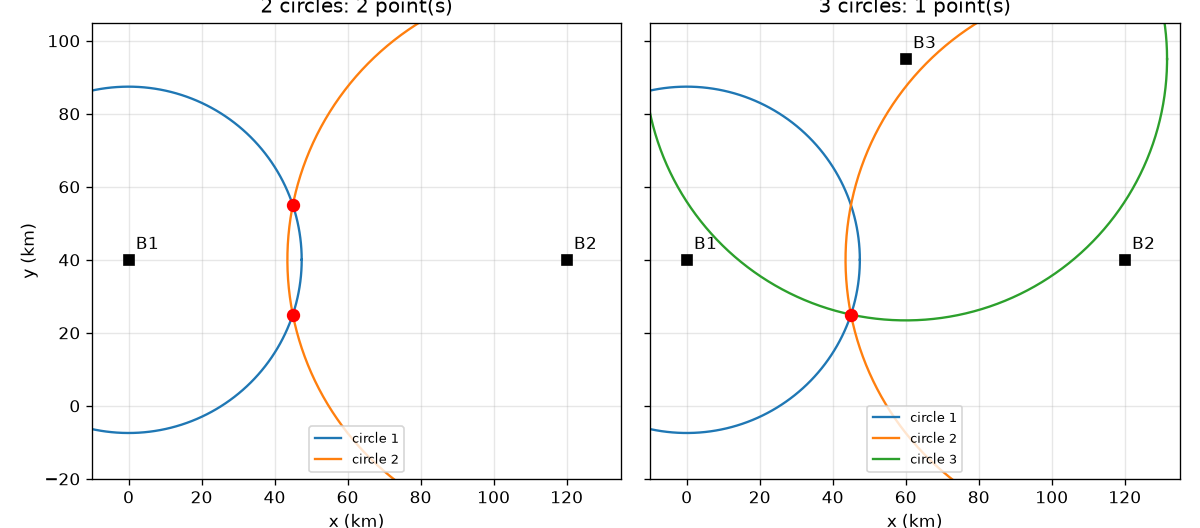
\includegraphics[width=0.85\linewidth]{figures/s01_circles_meet.png}\\\small Left: two circles meet at two points. Right: a third circle leaves one point (toy map, km).\end{center}

\subsection*{E. Worked example}
Beacons B1 = (0, 40), B2 = (120, 40), B3 = (60, 95) km. A receiver measures d1 = 47.43 km, d2 = 76.49 km and d3 = 71.59 km. Where is it?
\begin{enumerate}[nosep]
\item d = distance between B1 and B2 = 120 km. Squares of the ranges: r1\textasciicircum{}2 = 2250 and r2\textasciicircum{}2 = 5850 km\textasciicircum{}2.
\item a = (120\textasciicircum{}2 + 2250 - 5850) / (2 x 120) = 10800 / 240 = 45 km.
\item h = sqrt(2250 - 45\textasciicircum{}2) = sqrt(2250 - 2025) = sqrt(225) = 15 km.
\item The centres lie on the line y = 40, so the two candidates are (45, 40 - 15) = (45, 25) and (45, 40 + 15) = (45, 55) km.
\item Distance from (45, 55) to B3 is sqrt(15\textasciicircum{}2 + 40\textasciicircum{}2) = 42.72 km but r3 = 71.59 km, a miss of 28.87 km. Distance from (45, 25) to B3 is sqrt(15\textasciicircum{}2 + 70\textasciicircum{}2) = 71.59 km, a miss of zero.
\end{enumerate}
\textbf{Answer.} The receiver is at (45, 25) km; the other candidate (45, 55) km misses circle 3 by 28.87 km.

\subsection*{F. Questions}
\begin{enumerate}[nosep]
\item \textbf{Conceptual.} Why do two circles give two points and not one? What would a single extra circle have to avoid to be useful?
\item \textbf{Numerical.} A receiver is sqrt(4500) = 67.08 km from both B1 = (0, 40) and B2 = (120, 40). Find the two candidate positions. Then use B3 = (60, 95) with r3 = 25 km to choose.
\item \textbf{Graph and simulation interpretation.} In the distance graph (receiver moving along x at y = 25 km), where do the curves for B1 and B2 cross, and what is the distance there?
\item \textbf{Design and optimisation challenge.} Design: you can put the third beacon at (60, 40), (60, 95) or (130, 40) km, with B1 = (0, 40) and B2 = (120, 40). Which choices let a receiver at (45, 25) tell itself from its mirror image (45, 55)? Explain the trade-off.
\end{enumerate}

\section{Session 2: Distance is speed of light times time}

\subsection*{A. Real-world problem}
A GPS satellite sends a radio signal stamped with the time it left. Your phone notes when it arrives. The distance is the speed of light times the travel time, and light covers 300 m in a single microsecond. So how good must a clock be to locate you within 10 m? And how do we solve for a position from distances without solving quadratic equations? (Educational model with toy satellite positions, not real orbits; Earth is a sphere.)

\subsection*{B. Concept and theory}
A pseudorange is c times the measured travel time. It is called pseudo because the clocks are not perfect, so it is not exactly the true distance. Each satellite i at position s\_i gives \textbar{}x - s\_i\textbar{} = r\_i, a sphere (circle in 2D) around s\_i. Squares make this quadratic, but subtracting the equation of satellite 1 from satellite i cancels the \textbar{}x\textbar{}\textasciicircum{}2 term and leaves a plane (line in 2D): 2 (s\_i - s\_1) . x = \textbar{}s\_i\textbar{}\textasciicircum{}2 - \textbar{}s\_1\textbar{}\textasciicircum{}2 - r\_i\textasciicircum{}2 + r\_1\textasciicircum{}2. In 2D, three satellites give two such lines and a unique point. In 3D, three satellites give only two planes (two equations, three unknowns): their line of intersection cuts the first sphere in two points, so the answer is ambiguous; a fourth satellite adds a third plane and fixes it. A timing error dt is a range error c dt, and the position error is that range error multiplied by a geometry-dependent amplification.

\begin{itemize}[nosep]
\item c: speed of light in vacuum, 299,792,458 (m/s)
\item t: signal travel time (s)
\item r = c t: pseudorange (distance as the clock sees it) (m)
\item s\_i: position of satellite i (m)
\item x: receiver position (m)
\item dt: timing error (s)
\end{itemize}

\begin{equation*}
r_i=c\,t_i,\qquad \Delta r=c\,\Delta t
\end{equation*}

\begin{equation*}
\|\mathbf x-\mathbf s_i\|^2=r_i^2\ \Longrightarrow\ 2(\mathbf s_i-\mathbf s_1)\cdot\mathbf x=\|\mathbf s_i\|^2-\|\mathbf s_1\|^2-r_i^2+r_1^2
\end{equation*}

\begin{equation*}
A\mathbf x=\mathbf b,\qquad A=2\begin{pmatrix}(\mathbf s_2-\mathbf s_1)^{\mathsf T}\\ \vdots\\ (\mathbf s_n-\mathbf s_1)^{\mathsf T}\end{pmatrix}
\end{equation*}

\begin{equation*}
\Delta t_{\max}=\frac{\Delta r_{\max}}{c}
\end{equation*}

\begin{center}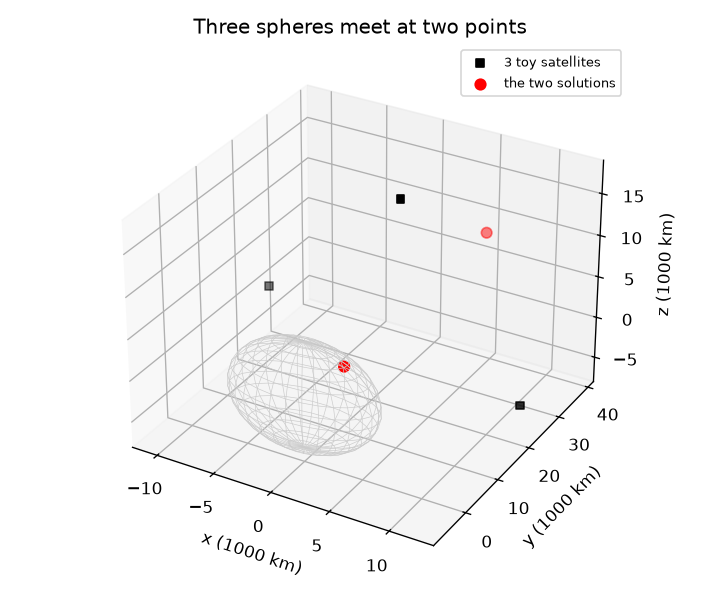
\includegraphics[width=0.85\linewidth]{figures/s02_three_spheres.png}\\\small Three toy satellites: the spheres meet at two points, one on the Earth, one far out in space.\end{center}

\subsection*{E. Worked example}
Three ground beacons B1 = (0, 40), B2 = (120, 40), B3 = (60, 95) km send timed signals to a receiver. It records travel times 158.22, 255.12 and 238.80 microseconds. Find the position by subtracting equations.
\begin{enumerate}[nosep]
\item Ranges r = c t: 158.22 us gives 47.43 km, 255.12 us gives 76.49 km, 238.80 us gives 71.59 km. So r1\textasciicircum{}2 = 2250, r2\textasciicircum{}2 = 5850, r3\textasciicircum{}2 = 5125 km\textasciicircum{}2.
\item Subtract equation 1 from equation 2: 2 (120, 0) . (x, y) = (14400 + 1600) - 1600 - 5850 + 2250, so 240 x = 10800 and x = 45 km.
\item Subtract equation 1 from equation 3: 2 (60, 55) . (x, y) = (3600 + 9025) - 1600 - 5125 + 2250, so 120 x + 110 y = 8150.
\item Put x = 45: 5400 + 110 y = 8150, so y = 25 km.
\item Check with equation 1: sqrt(45\textasciicircum{}2 + (25 - 40)\textasciicircum{}2) = sqrt(2250) = 47.43 km, which matches.
\end{enumerate}
\textbf{Answer.} The receiver is at (45, 25) km, the same as in Session 1. The clock accuracy for a 10 m range error is 10 / c = 33.4 nanoseconds.

\subsection*{F. Questions}
\begin{enumerate}[nosep]
\item \textbf{Conceptual.} Why does subtracting one sphere equation from another make the problem linear, and what do the new equations represent geometrically?
\item \textbf{Numerical.} A satellite clock is wrong by 50 nanoseconds. What range error is that? Is it small compared with a 10 m accuracy goal?
\item \textbf{Graph and simulation interpretation.} In the timing-error figure the position-error line is steeper than the range-error line. What does the ratio of slopes tell you, and what could make it larger?
\item \textbf{Design and optimisation challenge.} Design: you need the position error below 10 m, and in the toy geometry of the figure the amplification is about 2.14. How accurate (in nanoseconds) must the clock error on one range be? What steadiness over one day (a fraction) does that need?
\end{enumerate}

\section{Session 3: Solve for position and clock together, and check the geometry}

\subsection*{A. Real-world problem}
Your phone's clock is cheap: it can be off by milliseconds, and each millisecond is 300 km of range. So the phone treats its clock error as one more unknown, which is why GPS needs at least four satellites for a 3D fix. The ranges also have noise, and some satellite layouts give much better results than others. Finally, the satellites carry atomic clocks that run at a slightly different rate from clocks on the ground, because of relativity: how big is that, and what happens if nobody corrects it? (Educational model: toy satellite positions, not real orbits; no atmosphere, no real ephemeris; not a navigation tool.)

\subsection*{B. Concept and theory}
The model is rho\_i = \textbar{}s\_i - x\textbar{} + b + noise\_i, where b is the receiver clock error times c (in metres). The unknowns are z = (x, y, z, b). Gauss-Newton guesses z, predicts every rho\_i, and solves the linearised mismatch G dz = residual in the least-squares sense, where row i of G is [ -(s\_i - x)/\textbar{}s\_i - x\textbar{}, 1 ]. Repeating this converges in a few steps even from the Earth's centre. With equal noise sigma on every range, the covariance of the estimate is sigma\textasciicircum{}2 (G\textasciicircum{}T G)\textasciicircum{}-1; its diagonal gives the dilution of precision: PDOP is the factor by which the noise is multiplied in 3D position, so the expected rms position error is sigma x PDOP. A satellite clock is affected by relativity in two opposite ways. General relativity: higher in the gravity well the clock runs faster, by the fraction GM/c\textasciicircum{}2 (1/R\_earth - 1/r\_sat). Special relativity: a moving clock runs slower, by v\textasciicircum{}2/(2 c\textasciicircum{}2), with v\textasciicircum{}2 = GM/r\_sat for a circular orbit. These are well-known approximate results; we compute them below with a spherical Earth and ignore smaller effects (Earth's rotation, orbit eccentricity).

\begin{itemize}[nosep]
\item x: receiver position (m)
\item b = c x (clock error): receiver clock bias as a distance (m)
\item rho\_i: measured pseudorange to satellite i (m)
\item sigma: range noise (standard deviation) (m)
\item G: geometry matrix, rows [-unit vector to satellite, 1] (no unit)
\item PDOP, HDOP, VDOP, TDOP: dilution of precision (3D, horizontal, vertical, time) (no unit)
\item GM: Earth's gravitational parameter 3.986004418e14 (m\textasciicircum{}3/s\textasciicircum{}2)
\item R\_earth, r\_sat: 6,371,000 and 26,560,000 (toy) (m)
\end{itemize}

\begin{equation*}
\rho_i=\|\mathbf s_i-\mathbf x\|+b+\varepsilon_i
\end{equation*}

\begin{equation*}
G\,\delta\mathbf z=\boldsymbol\rho-\hat{\boldsymbol\rho}(\mathbf z),\qquad G_i=\left[-\frac{(\mathbf s_i-\mathbf x)^{\mathsf T}}{\|\mathbf s_i-\mathbf x\|},\ 1\right]
\end{equation*}

\begin{equation*}
Q=(G^{\mathsf T}G)^{-1},\qquad \mathrm{PDOP}=\sqrt{Q_{11}+Q_{22}+Q_{33}},\qquad \text{rms error}\approx\sigma\,\mathrm{PDOP}
\end{equation*}

\begin{equation*}
\frac{\Delta f}{f}\Big|_{\rm gravity}=\frac{GM}{c^2}\left(\frac{1}{R_E}-\frac{1}{r_s}\right),\qquad \frac{\Delta f}{f}\Big|_{\rm motion}=-\frac{v^2}{2c^2}=-\frac{GM}{2c^2 r_s}
\end{equation*}

\begin{center}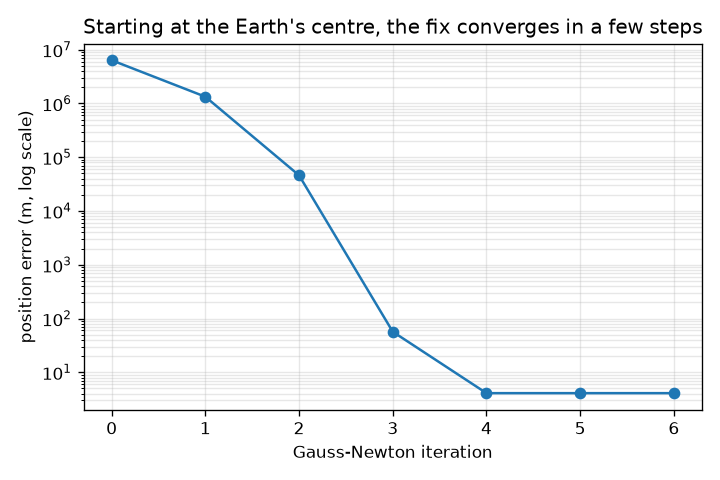
\includegraphics[width=0.85\linewidth]{figures/s03_convergence.png}\\\small Error of the fix at each Gauss-Newton iteration, starting from the Earth's centre.\end{center}

\subsection*{E. Worked example}
Compute the relativity offsets of a GPS satellite clock at r = 26,560 km from the Earth's centre (ground at 6371 km), and the range error if left uncorrected for one day.
\begin{enumerate}[nosep]
\item GM/c\textasciicircum{}2 = 3.986004e14 / 8.98755e16 = 4.4350e-3 m. 1/R\_E = 1.5696e-7 per m and 1/r\_s = 3.7651e-8 per m, so the difference is 1.1931e-7 per m.
\item Gravity: fractional rate = 4.4350e-3 x 1.1931e-7 = 5.2915e-10. Per day: 5.2915e-10 x 86400 s = 4.572e-5 s = +45.7 microseconds per day (the clock runs fast).
\item Motion: v\textasciicircum{}2 = GM / r\_s = 1.5008e7 m\textasciicircum{}2/s\textasciicircum{}2 (v = 3874 m/s). Fraction = v\textasciicircum{}2 / (2 c\textasciicircum{}2) = 8.349e-11. Per day: 7.21 microseconds, with a minus sign (the clock runs slow).
\item Net = 45.7 - 7.2 = +38.5 microseconds per day (the clock runs fast).
\item Range: c x 38.5e-6 s = 11.5 km per day. After 10 days: 115 km.
\end{enumerate}
\textbf{Answer.} About +45.7 (gravity) and -7.2 (motion), net +38.5 microseconds per day; left uncorrected, about 11.5 km of range per day. These match the well-known approximate values (about 45, 7 and 38 microseconds per day). Even if every satellite clock shared the error, the receiver bias absorbs it (the checkpoint shows this); but the error would still spoil time transfer, and any clock that differs from the others (one wrong clock) moves the fix, by 22.0 km in our four-satellite example after one day.

\subsection*{F. Questions}
\begin{enumerate}[nosep]
\item \textbf{Conceptual.} Why does a 3D GPS fix need four satellites even when the satellites are known exactly and the Earth's radius is known?
\item \textbf{Numerical.} Range noise has sigma = 3 m and the satellites give PDOP = 3.48. What rms 3D position error do you expect? And with PDOP = 1.89?
\item \textbf{Graph and simulation interpretation.} In the DOP-validation figure the dots lie on the line sigma x PDOP. What does that say about the simulation and about DOP? What would it mean if the dots were far above the line?
\item \textbf{Design and optimisation challenge.} Design: a phone has eight toy satellites in view but can use only four. There are 70 choices. Which four would you use, and why? What does the worst four do?
\end{enumerate}

\section{Real-world mini-project}
\textbf{Locate a phone from satellite ranges.} A phone tracks eight toy satellites but its chip can use only four at a time. The synthetic pseudoranges are made in code with \texttt{pseudoranges(sats, rec, bias, 5.0, np.random.default\_rng(2024))} using the receiver at 19 N, 73 E, \texttt{GOOD\_SKY} satellites and a clock bias of 0.35 ms. Find the best four satellites (lowest PDOP) out of the 70 possible sets, fix the phone with them using \texttt{gauss\_newton}, and compare with the first four satellites.

\section{The path ahead}
\begin{enumerate}[nosep]
\item \textbf{Session 4: Real orbits instead of fixed toy positions.} An orbit propagator that gives each satellite position at any time, replacing the fixed toy positions.
\item \textbf{Session 5: Atmosphere delay.} A delay model added to the simulated ranges and a correction in the solver.
\item \textbf{Session 6: Weight the satellites.} A weighted Gauss-Newton solver with elevation-dependent noise.
\item \textbf{Session 7: Detect and exclude a faulty satellite.} A fault detector that flags and removes one bad range.
\item \textbf{Session 8: Velocity from Doppler.} A second linear solve for the velocity and clock drift of a moving receiver.
\end{enumerate}

\section{Answers and hints}

\subsection*{Session 1}
\begin{enumerate}[nosep]
\item \textbf{Conceptual.} Hint: Think of the line joining the two centres and a mirror placed on it. Solution: If a point is at distance r1 from c1 and r2 from c2, its mirror image across the line through c1 and c2 has exactly the same two distances, so both are valid answers. A third circle helps only if its centre is NOT on that line: otherwise the mirror image is at the same distance from it too and the ambiguity remains.
\item \textbf{Numerical.} Hint: d = 120 km, so a = d/2 when r1 = r2. Then h = sqrt(r1\textasciicircum{}2 - a\textasciicircum{}2). Solution: a = (14400 + 4500 - 4500) / 240 = 60 km and h = sqrt(4500 - 3600) = sqrt(900) = 30 km, so the candidates are (60, 70) and (60, 10) km. Distance from (60, 70) to B3 is 25 km, which matches r3; from (60, 10) it is 85 km. The fix is (60, 70) km. Sanity check: 60 is halfway between x = 0 and x = 120, as it must be for equal distances.
\item \textbf{Graph and simulation interpretation.} Hint: They cross where the two distances are equal. B1 and B2 sit at x = 0 and x = 120. Solution: They cross at x = 60 km, halfway between the beacons, where each distance is sqrt(60\textasciicircum{}2 + 15\textasciicircum{}2) = sqrt(3825) = 61.85 km. Left of 60 the receiver is closer to B1, right of 60 closer to B2.
\item \textbf{Design and optimisation challenge.} Hint: The mirror line is y = 40. A beacon on that line is equally far from both candidates. Solution: (60, 40) and (130, 40) lie on the line y = 40 so they are equally far from (45, 25) and (45, 55): they cannot decide. Only (60, 95) works (distance 71.59 km versus 42.72 km). A beacon far off the line gives a large difference between the two candidates, so the choice is robust to ranging errors: the gap here is 28.87 km. A beacon only slightly off the line would give a tiny difference and an error of a few hundred metres could pick the wrong point.
\end{enumerate}

\subsection*{Session 2}
\begin{enumerate}[nosep]
\item \textbf{Conceptual.} Hint: Write \textbar{}x - s\textbar{}\textasciicircum{}2 = \textbar{}x\textbar{}\textasciicircum{}2 - 2 s.x + \textbar{}s\textbar{}\textasciicircum{}2 and look at the \textbar{}x\textbar{}\textasciicircum{}2 terms. Solution: Expanding \textbar{}x - s\_i\textbar{}\textasciicircum{}2 = r\_i\textasciicircum{}2 gives \textbar{}x\textbar{}\textasciicircum{}2 - 2 s\_i.x + \textbar{}s\_i\textbar{}\textasciicircum{}2 = r\_i\textasciicircum{}2. The term \textbar{}x\textbar{}\textasciicircum{}2 is the same in every equation, so it cancels when we subtract two of them, leaving something linear in x. Each such equation is a plane (line in 2D): the plane containing all points that are on both spheres, which is where the two spheres cross.
\item \textbf{Numerical.} Hint: range error = c x timing error; 50 ns = 50e-9 s. Solution: 299,792,458 m/s x 50e-9 s = 14.99 m, about 15 m. That alone already exceeds the 10 m goal, before any amplification by geometry. Sanity check: 1 microsecond is 300 m, so 50 ns = 1/20 of that = 15 m.
\item \textbf{Graph and simulation interpretation.} Hint: Slope = metres of error per microsecond of timing error. Solution: The slopes are about 642 m per microsecond (position) and 299.8 m per microsecond (range): the ratio, about 2.1, is the amplification of range error into position error by this geometry. Satellites bunched close together in the sky make it larger (the app shows about 11 at its narrowest 20 degree spread, and below 1 at 85 degrees); satellites spread widely make it smaller.
\item \textbf{Design and optimisation challenge.} Hint: Position error = 642.4 m per microsecond of timing error. Divide the allowed error by it. Then divide by the number of seconds in a day, 86,400. Solution: 10 m / 642.4 m per microsecond = 0.01557 microseconds = 15.6 ns. Holding 15.6 ns over one day needs a fractional steadiness of 15.6e-9 / 86400 = 1.8e-13. (If the geometry did not amplify, 10 m would need 33.4 ns and 3.9e-13.) This is why GPS satellites carry atomic clocks, and a phone's cheap clock is not good enough: Session 3 solves for the phone's clock error instead. Trade-off: better clocks cost more; better geometry costs nothing but depends on where the satellites are.
\end{enumerate}

\subsection*{Session 3}
\begin{enumerate}[nosep]
\item \textbf{Conceptual.} Hint: Count the unknowns in z, and ask what the receiver clock does to every pseudorange. Solution: There are four unknowns: x, y, z and the receiver clock bias b. The cheap receiver clock adds the same unknown distance b to every pseudorange, so each satellite gives one equation and four equations are needed. (Earth-radius knowledge could replace one satellite but only if the receiver is known to be on the surface.)
\item \textbf{Numerical.} Hint: rms error is about sigma x PDOP. Solution: 3 x 3.48 = 10.4 m for PDOP 3.48 and 3 x 1.89 = 5.7 m for PDOP 1.89. Sanity check: the error is a few times the noise, and better geometry (lower PDOP) reduces it.
\item \textbf{Graph and simulation interpretation.} Hint: The line is the theory; the dots are measured rms errors from many noisy fixes. Solution: The simulation agrees with the theory, so DOP correctly predicts how much geometry multiplies range noise. Dots far above the line would mean something else is adding error (an unmodelled bias, a faulty satellite, or Gauss-Newton failing to converge), so the fix is worse than the geometry alone explains.
\item \textbf{Design and optimisation challenge.} Hint: Compute PDOP for every set of four with \texttt{dop} and compare. Do not forget to inspect the worst set. Solution: The best set is satellites 4, 5, 6 and 7 (1-indexed), with PDOP 2.55, versus 3.48 for the first four. The worst set (satellites 2, 3, 4, 5) has PDOP 363.7: a tiny noise is multiplied by hundreds and Gauss-Newton may even diverge. Choose by PDOP; the trade-off is that the best geometry may include low satellites that suffer more atmosphere delay in the real world, which this model leaves out.
\end{enumerate}

\section{How to join}
Read \texttt{CONTRIBUTING.md} in the repository, then pick an issue labelled \texttt{good first issue}. Repository: \url{https://github.com/KrunalPanchal1995/opengps}

\end{document}
